\documentclass[12pt]{IEEEtran}
\usepackage{graphicx}
\begin{document}
\title{\textbf{Dialogue Generation using Transformer's GPT-2 Model }}
\author{{Shahryar Akbar 22I-0074 Intikhab Mehdi 22I-1434}

\emph{Masters in Data Science}

\emph{FAST NUCES, Islamabad}}
\maketitle
\begin{abstract}
Dialogue generation is an important aspect of natural language processing that has practical applications in chatbots, virtual assistants, and entertainment. In this paper, we explore the use of a pre-trained Hugging Face GPT-2 model for generating dialogues. Gpt-2 model is fine tuned on Empathetic Dialogues dataset so that the model captures the emotions of natural human language, we propose a method that generates dialogues based on random user inputs. Our approach leverages the GPT-2's pre-trained data and self-attention mechanism to generate coherent and contextually relevant dialogues.Our experimental results demonstrate that our method produces high-quality dialogues that are not only contextually correct but also offers emotional support in the model's output responce. Overall, our work contributes to the advancement of dialogue generation using pre-trained language models and opens up new avenues for exploring the potential of these models in conversational AI.
\end{abstract}
\section{Introduction}\label{sectionintro}
Transformers have become a dominant architecture for natural language processing (NLP) tasks in recent years, due to their exceptional performance and ability to capture long-range dependencies. Transformers are a type of deep learning model architecture that have revolutionized the field of natural language processing (NLP). They were introduced in the seminal paper "Attention Is All You Need" by Vaswani et al. \cite{attention} in 2017. Unlike traditional recurrent neural networks (RNNs) that process language sequentially, transformers can capture long-range dependencies in text by employing a self-attention mechanism. The key idea behind transformers is the concept of attention, which allows the model to focus on different parts of the input sequence when processing each word or token. This attention mechanism enables the model to weigh the importance of different words or tokens in the context of the entire sequence, thereby capturing contextual relationships more effectively. This parallelization and attention-based approach make transformers highly efficient and capable of modeling complex language patterns.
Hugging Face is an organization that has gained significant recognition for its contributions to the NLP community. They have developed a library called "Transformers" that provides a user-friendly and comprehensive interface for working with state-of-the-art transformer models. The Hugging Face Transformers library offers a wide range of pre-trained models, including GPT-2, BERT, RoBERTa, and many others, which can be easily utilized for various NLP tasks such as text classification, named entity recognition, question answering, and, of course, dialogue generation.
The Hugging Face Transformers library simplifies the process of using pre-trained transformer models by providing a unified API that allows researchers and developers to fine-tune these models on their specific tasks and datasets. The library offers ready-to-use tokenizers, model architectures, and training utilities, making it easier to experiment with and apply transformer models in practice. In the context of dialogue generation, Hugging Face's Transformers library provides a convenient framework to fine-tune pre-trained transformer models like GPT-2 on dialogue datasets. Researchers can leverage the power of these models and the extensive functionality provided by the library to develop sophisticated dialogue generation systems with human-like responses
Dialogue generation, a prominent subfield of natural language processing (NLP), focuses on the development of automated systems that can generate human-like conversations. It plays a vital role in various applications, including virtual assistants, chatbots, customer service agents, and interactive storytelling. Effective dialogue generation models have the potential to revolutionize human-computer interactions and enhance user experiences.
\subsection{Background}
One significant advancement in dialogue generation has been the utilization of pre-trained models. Pre-trained models are neural network architectures that have been trained on vast amounts of data, allowing them to learn intricate patterns and structures of language. These models capture the syntactic and semantic nuances of human speech, enabling them to generate coherent and contextually appropriate responses. The introduction of pre-trained models has significantly improved the efficiency and quality of dialogue generation. These models, when fine-tuned for dialogue tasks, offer a head start by leveraging their pre-existing knowledge of language. They learn from large-scale corpora, including internet text, books, and articles, capturing diverse language patterns and contextual information. Consequently, pre-trained models provide a foundation for dialogue generation systems to produce more coherent, natural, and contextually appropriate responses.
One such pre-trained model that has gained significant attention is the Generative Pre-trained Transformer 2 (GPT-2). GPT-2 is a state-of-the-art language model developed by OpenAI, characterized by its ability to generate high-quality text that resembles human writing. GPT-2 employs a transformer architecture, which enables it to capture long-range dependencies in text and generate coherent and contextually consistent responses.
The capabilities of GPT-2 in generating human-like dialogue have made it a popular choice for dialogue generation research. By fine-tuning GPT-2 on dialogue datasets and employing various techniques, researchers have achieved impressive results in generating interactive and engaging conversations. GPT-2's ability to understand and mimic the conversational style, tone, and context of human dialogue has paved the way for advancements in dialogue systems.
\subsection{objective}
In this research paper, we delve into the realm of dialogue generation using the pre-trained Hugging Face Transformer model GPT-2. We explore the methodology, experimental setup, and results of using pre-trained GPT-2 to generate dialogues, aiming to generate human-like responses in conversational settings. By examining the performance and limitations of GPT-2, we contribute to the understanding of pre-trained models' effectiveness in dialogue generation and highlight the potential impact of such models in various applications.
The following sections of this paper discuss related work, methodology, results, and analysis, providing valuable insights into the capabilities and challenges of dialogue generation using GPT-2. Through this research, we aim to shed light on the advancements, limitations, and future directions in the field of dialogue generation and its association with pre-trained models like GPT-2.








\section{Literature Review}
Natural language processing has seen a significant surge in recent years due to the availability of large amounts of data and advancements in deep learning techniques. One of the key areas of natural language processing is text generation, which involves generating text based on some given input or context. The OpenAI GPT-2 and BERT models have emerged as widely used language models for text generation and prediction.GPT-2 is a generative language model that uses a transformer-based architecture to generate text. It has been pre-trained on a large corpus of data and can be fine-tuned for specific text generation tasks. BERT, on the other hand, is a bidirectional language model that uses a transformer-based architecture to predict masked words in a sentence. There have been many experiments conducted to verify the outstanding performance of these two models in the field of text generation. The paper "A Text Generation and Prediction System: \cite{Gpt-2_text} Pre-training on New Corpora Using BERT and GPT-2" proposes a new approach to pre-train GPT-2 on two new corpora, BaiduBaike and LLKT, to generate long sentences and articles. The authors collected a large amount of data from BaiduBaike and the LeLeKeTang website and filtered out short data that may affect the generation effect. They pre-trained the GPT-2 model on this data and used it to generate long sentences and articles. They also used the BERT model to complete the task of predicting intermediate words based on the context. Through experimental results, the authors showed that GPT-2 and BERT models perform well in text generation tasks. However, they noted that there are still some shortcomings, such as readability, corpora data, and training methods, which may cause generated sentences to be repeated, among others. In conclusion, the paper proposes a new approach to pre-train GPT-2 on new corpora for text generation tasks. The authors demonstrate the effectiveness of their approach through experimental results and highlight the potential limitations of current language models. The paper provides insights for researchers interested in text generation and natural language processing.
Emotion style transfer has been an emerging area of research in natural language processing (NLP) over the past few years. With the increasing popularity of transformer-based language models, researchers have been exploring ways to leverage these models to perform emotion style transfer. Recent studies have proposed various approaches to emotion style transfer, including supervised and unsupervised methods. Supervised approaches rely on labeled data to train the model, while unsupervised approaches do not require labeled data and instead use generative models to transfer emotions.  One of the most popular generative models used for this task is the GPT-2 model, which has shown impressive results in various NLP tasks. However, previous research has not explored the use of GPT-2 for emotion style transfer. In addition to emotion style transfer, paraphrasing has also been an area of interest in NLP. Various models have been proposed for paraphrasing, including sequence-to-sequence models and transformers. These models have shown promising results in generating paraphrases that maintain the meaning of the original sentence while improving its fluency and readability.  In this paper \cite{emotion}, the authors propose a system that combines the power of GPT-2 and a paraphrasing model for emotional paraphrasing. The authors fine-tune a GPT-2 model with corrupted emotional data to increase the emotional intensity of the input sentence. This is coupled with a paraphrasing model to generate a paraphrase that also conveys the same emotion as the original sentence.  The authors conducted a qualitative study with human judges and a quantitative evaluation to assess the effectiveness of their system. Although the paraphrase metrics show poor performance compared to the state of the art, the transfer of emotion proved to be effective, especially for the emotions fear, sadness, and disgust. The perception of these emotions were improved both in the automatic and human evaluations. Overall, the proposed system has potential to facilitate the automatic creation of training sentences for NLU systems, as well as integrate into emotional or empathic dialogue architectures.
Biomedical text processing has become an important area of research in natural language processing (NLP), particularly with the increasing amount of electronic health records (EHRs) being generated. Recent advancements in contextual word embeddings and Transformer-based models have shown great potential in various NLP tasks, but there is a lack of resources available for low-resource languages like Portuguese. In this paper \cite{por}, the authors aim to address this issue by developing a Generative Pre-trained Transformer 2 (GPT-2) language model for Portuguese biomedical texts through transfer learning. Several studies have focused on developing NLP models for English biomedical texts, but there is a need for similar research in low-resource languages like Portuguese. Existing studies have shown the effectiveness of transfer learning in improving the performance of NLP models in biomedical tasks. The authors of this paper build on this research by fine-tuning a generic Portuguese GPT-2 model to corpora of biomedical texts in Portuguese using transfer learning. The authors evaluate their model on a public dataset manually annotated for detecting patient falls and compare its performance with the generic Portuguese GPT-2 model. The results show that the in-domain GPT-2 model outperforms the generic model by a significant margin in F1-score (weighted). These preliminary results demonstrate the potential of transfer learning with domain literature to improve the performance of Portuguese biomedical NLP models, which can have significant implications in improving healthcare outcomes in Portuguese-speaking regions.
\section{Research Methodology and Model}
GPT-2 is a generative language model developed by OpenAI that uses deep learning to generate human-like text. It is a neural network architecture that is trained on a large corpus of text and can then generate new text based on the input it receives. The architecture of GPT-2 is based on the transformer model, which was introduced by Vaswani et al. in 2017. The transformer model is a neural network architecture that uses self-attention to process sequences of input data. Self-attention is a mechanism in deep learning models that allows them to weigh the importance of different parts of the input sequence when making predictions. In natural language processing tasks, it has become an essential component of many state-of-the-art models, including GPT-2.
The self-attention mechanism in GPT-2 allows the model to analyze each word in a sequence while considering the relationships between all the other words in the sequence. This is achieved by transforming each word into a query, a key, and a value, which are then used to calculate the attention scores between each word and all the other words in the sequence.
The self-attention calculation is performed in three steps
Query, Key, Value Transformations: Each word in the sequence is transformed into a query, key, and value vector by multiplying it with learned weight matrices. These vectors represent the word's information in different contexts.
Attention Scores: The dot product of the query and key vectors is taken to produce the attention scores for each word in the sequence. This step allows the model to determine which words in the sequence are most relevant to each other.
Weighted Sum: The attention scores are normalized using a softmax function to obtain weights, which are then used to compute a weighted sum of the value vectors. This final vector is the output of the self-attention mechanism and represents the contextualized representation of the original word.
By repeating this process for each word in the sequence, GPT-2 can learn complex relationships and dependencies between words in a text. This allows it to generate coherent and contextually appropriate responses in dialogue generation tasks.
\begin{figure}[htp]
  \centering
  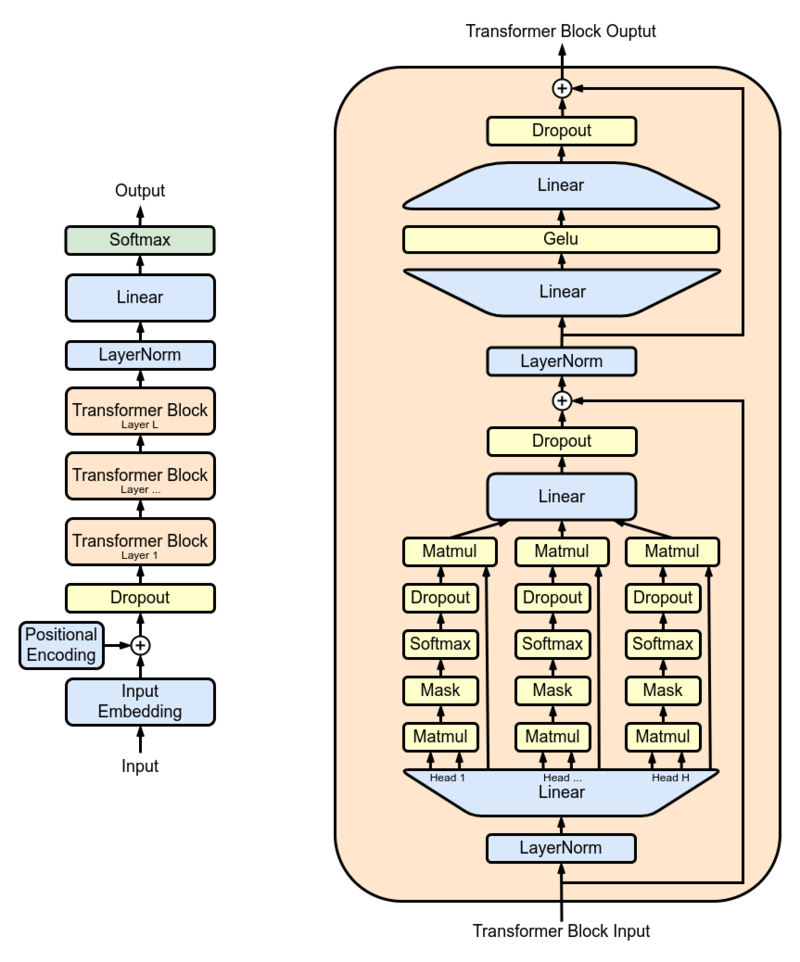
\includegraphics[width=9cm]{1.png}
  \caption{The GPT architecture}\label{figuregpt-2model}
\end{figure}
GPT-2, the transformer model employed in this research, offers a specialized architecture tailored for language modeling tasks. It comprises 12 layers of transformer blocks and has undergone training on an extensive dataset consisting of over 8 million web pages. The dataset's vast size, coupled with GPT-2's self-attention mechanism, empowers the model to capture an extensive range of language patterns and styles. During training, GPT-2 learns to predict the subsequent word in a given sequence by processing sequences of text. This unsupervised learning approach enables the model to make predictions without explicit instruction on the correct answers. Consequently, once trained, the model can generate new text by providing it with an initial prompt. By leveraging its learned probabilities for the next word, GPT-2 generates text incrementally, word by word. To ensure high-quality text generation, GPT-2 utilizes a technique called "top-k sampling," which limits the consideration of the top k most likely words at each step. This strategy enhances coherence and meaning in the generated text. It is important to note that GPT-2's training data encompasses a diverse range of text sources, including news articles, books, and web pages. The intention behind this diversity is to equip the model with the ability to generate text representative of various writing styles and subjects. The utilization of GPT-2 in fine-tuning on an empathetic dialogue dataset enables the model to generate empathetic responses that reflect a deep understanding of human emotions and experiences, further enhancing its language generation capabilities.
\begin{figure}[htp]
  \centering
  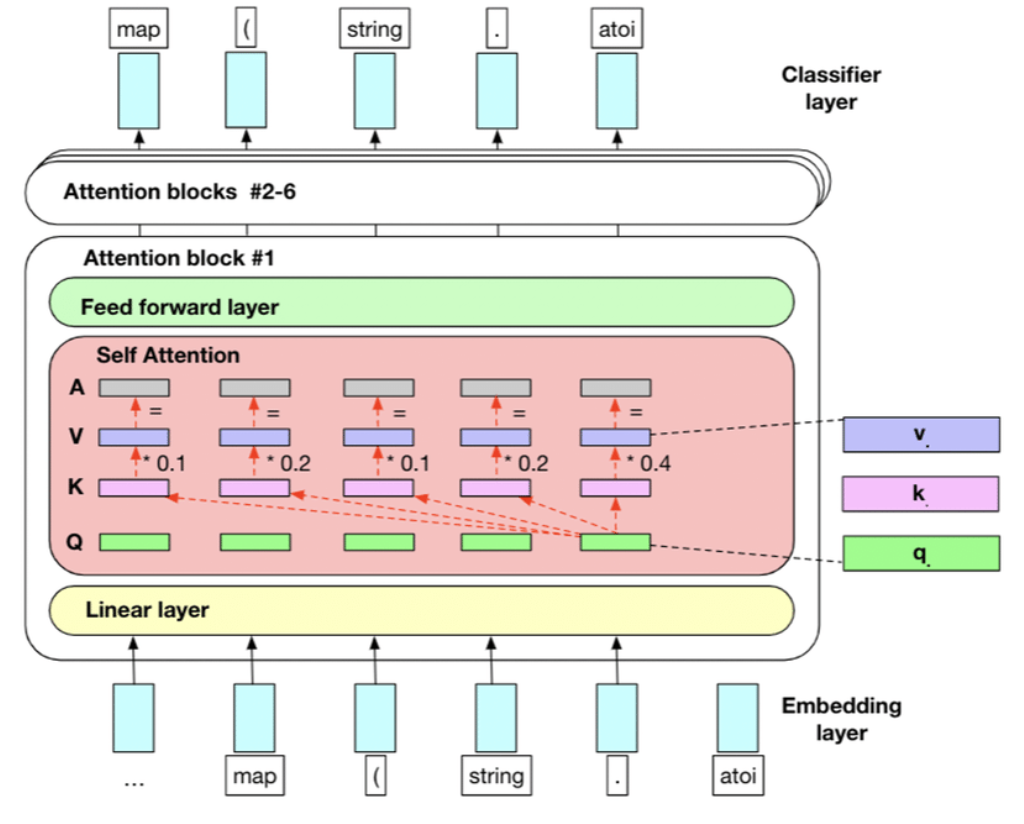
\includegraphics[width=8cm]{2.png}
  \caption{Architecture of the GPT-2 Transformer model}\label{figuregpt-2model}
\end{figure}

\subsection{Data}
In our research paper, we utilized a dataset consisting of dialogues with associated emotions and empathetic responses for the fine-tuning of our GPT-2 model. The dataset captures various situations and emotions expressed by individuals, providing a rich context for training the dialogue generation model. The dataset comprises several dialogue samples, each characterized by a situation, an emotion, empathetic dialogues, and corresponding labels. Let's examine a few examples from the dataset:

\textbf{Example :}
\emph{Situation: "I remember going to the fireworks with my best friend.There were a lot of people, but it only felt like us in the world."}

\emph{Emotion: Sentimental}

\emph{Empathetic Dialogues:
- Customer: "I remember going to see the fireworks with my best friend. It was the first time we ever spent time alone together. Although there were a lot of people, we felt like the only people in the world."
- Agent: "Was this a friend you were in love with, or just a best friend?"}


This example illustrate the diversity of situations, emotions, and empathetic responses present in the dataset. The dataset encompasses various sentimental situations, such as reminiscing about past experiences, missing a friend, and reflecting on changing relationships. It also covers emotions like fear and the associated dialogue expressing the individual's perspective. Each dialogue instance consists of a customer's statement followed by an empathetic response from the agent. The empathetic responses aim to acknowledge and understand the customer's emotions, providing supportive or inquisitive follow-up statements. The labels associated with each dialogue instance indicate the appropriate empathetic response based on the situation and emotion expressed. By utilizing this dataset for fine-tuning our GPT-2 model, we aimed to train the model to generate empathetic and contextually appropriate responses in dialogue scenarios. The dataset's variety of situations, emotions, and empathetic dialogues provided a diverse and representative training environment, enabling our model to learn to respond empathetically and effectively to a wide range of user inputs.
Overall, the dataset served as a valuable resource for training and evaluating our dialogue generation model, facilitating the exploration of empathy in automated conversational systems.

\section{Limitations and Future Work}
It is essential to acknowledge the limitations and challenges encountered during our research. While GPT-2 excels at generating coherent and contextually appropriate responses, it sometimes lacks factual accuracy and can produce nonsensical, repetitive and biased content. The model's reliance on pre-existing data and its inability to reason or understand context beyond its training data are areas that require further exploration and improvement. Looking ahead, future research could focus on enhancing GPT-2's performance by incorporating additional fine-tuning techniques on a more diverse and large dataset or employing more sophisticated methods for dialogue generation. Exploring ways to improve factual accuracy, controlling response diversity, and mitigating biases in generated dialogues are vital directions for advancement.
\section{Conclusion}
In this research paper, we explored the application of the pre-trained Hugging Face Transformer model GPT-2 for dialogue generation. By utilizing GPT-2's powerful language modeling capabilities, we were able to generate contextually relevant and human-like responses based on an initial dialogue input. Our experimentation with GPT-2 demonstrated its ability to capture the intricacies of language and generate coherent and contextually appropriate dialogue. The model showcased a remarkable capacity to understand the conversational style, tone, and context of the input dialogue, leading to the production of responses that closely resembled human-generated conversation. By leveraging the strengths of GPT-2's pre-training on vast amounts of diverse text data, we harnessed the power of transfer learning in dialogue generation. This enabled us to achieve impressive results by fine-tuning GPT-2 on Empathetic Dialogues dataset. The utilization of pre-trained models like GPT-2 significantly reduces the computation requirements for dialogue generation, making it a more accessible and efficient approach.

\bibliographystyle{ieeetr}
\bibliography{me}
\end{document} 